
It is a phenomenon we may encounter when we try to align two functions without a
perfect match taking the $\mathbb{L}^2$ distance as energy. To minimize the term
energy, the optimal solution will tend to
squeeze an annoying region, until it disappears. Figure \ref{FIG:PINCHING}
shows the result of the registration of two functions with pinching effect.
A part of $f_2$ is identical to $f_1$ over [0, 0.6] and completely different
over the remaining domain. The optimal solution will tend to squeeze the second
part of $f_2$, until it vanishes completely.

\begin{figure}[Pinching force effect]{FIG:PINCHING}{Pinching force effect}
	\subfigure[SBFIG:PINCHING1]{ $f_1$ and $f_2$}{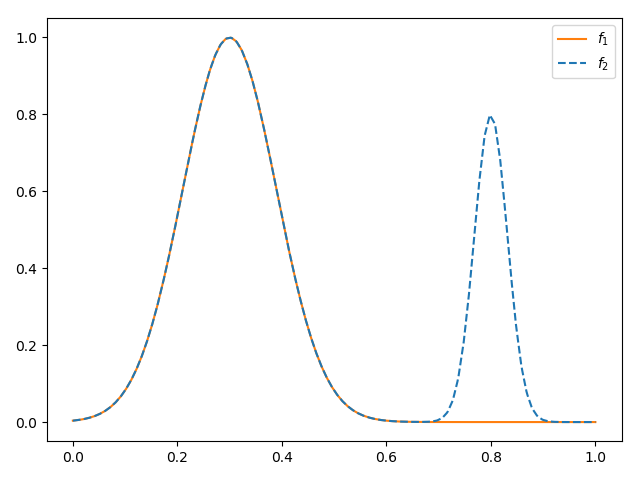
\includegraphics[width=7.5cm]{pinching-dataset}} \quad
	\subfigure[SBFIG:PINCHING2]{Pinching effect}{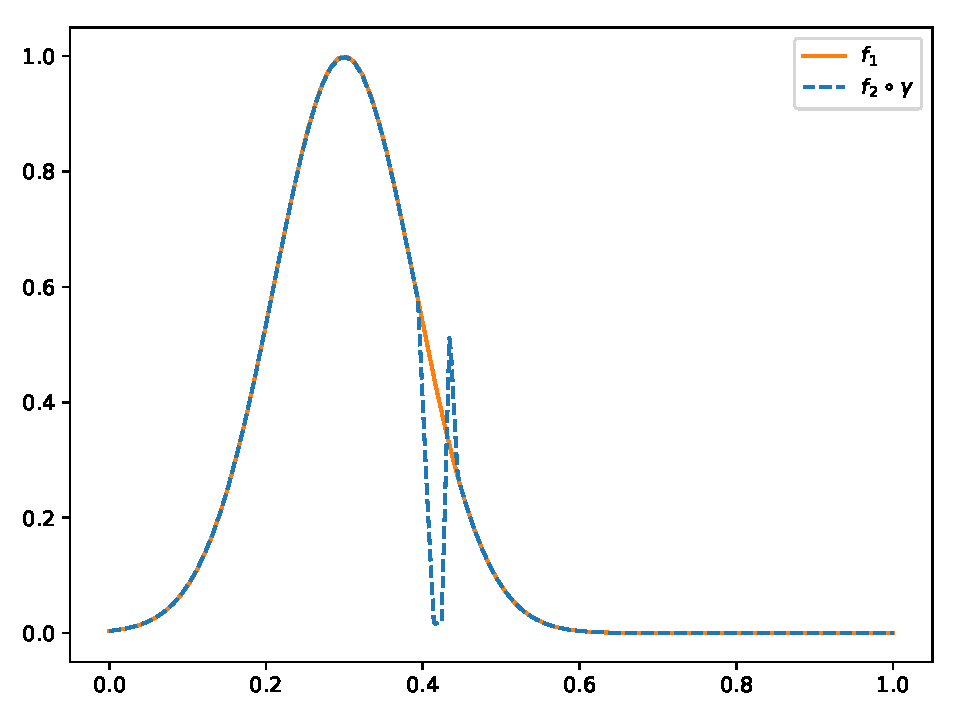
\includegraphics[width=7.5cm]{pinching-effect}}
\end{figure}